\section{Discussion}
\subsection{Overview}
It is rather obvious that deep learning algorithms fared much better at this task than the more basic machine learning algorithms such as Random Forests, or Stochastic gradient. The masks generated by the UNET algorithm are good enough that some postprocessing (closing the image or opening it) significantly improve it's IoU .
\subsection{Random Forests}
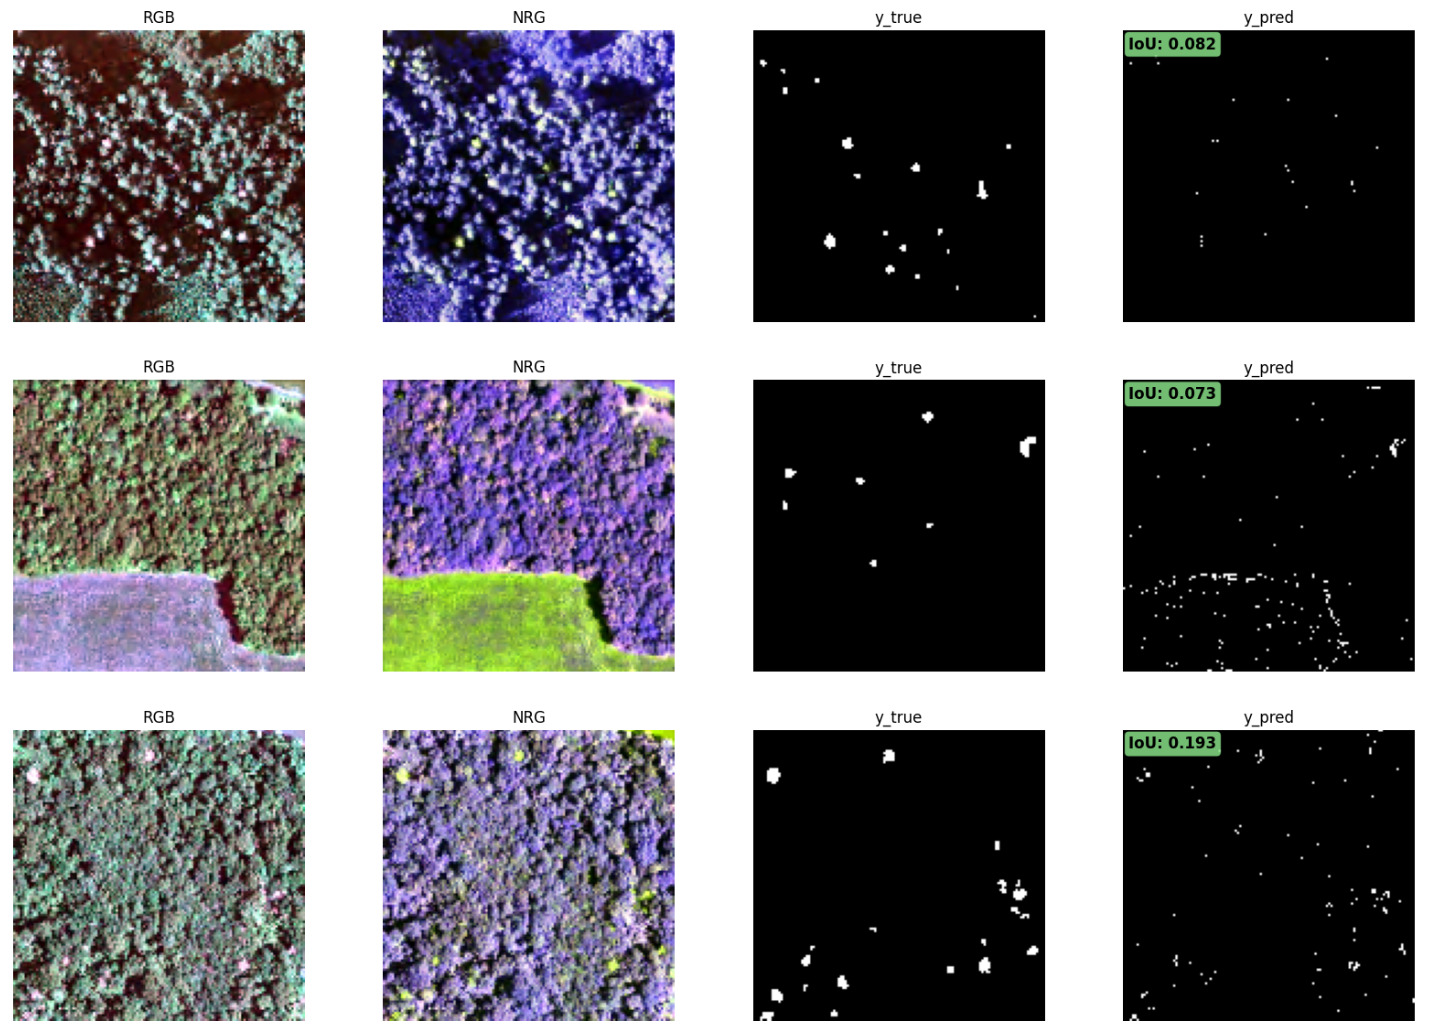
\includegraphics[width=.95\linewidth]{figs/RFmask.jpg}\\
When we look at the masks produced by the random forest, we can see that part of the reason for the poor performance is due to it reacting to spots where there are no trees, and due to the mask being far too small at spots where there is a dead tree, but the mask did detect almost all of the dead tree spots.  Likely what is happening is the RF determines each pixel to be a dead tree based on its colour, which would result in this behaviour. This is probably due to the random forest implementation being independent of location (the pixel information was passed to the random forest with no information of what it was nearby). this would likely be improved by the kernel based RF implementation, as described in the methods section.
\subsection{SGD}
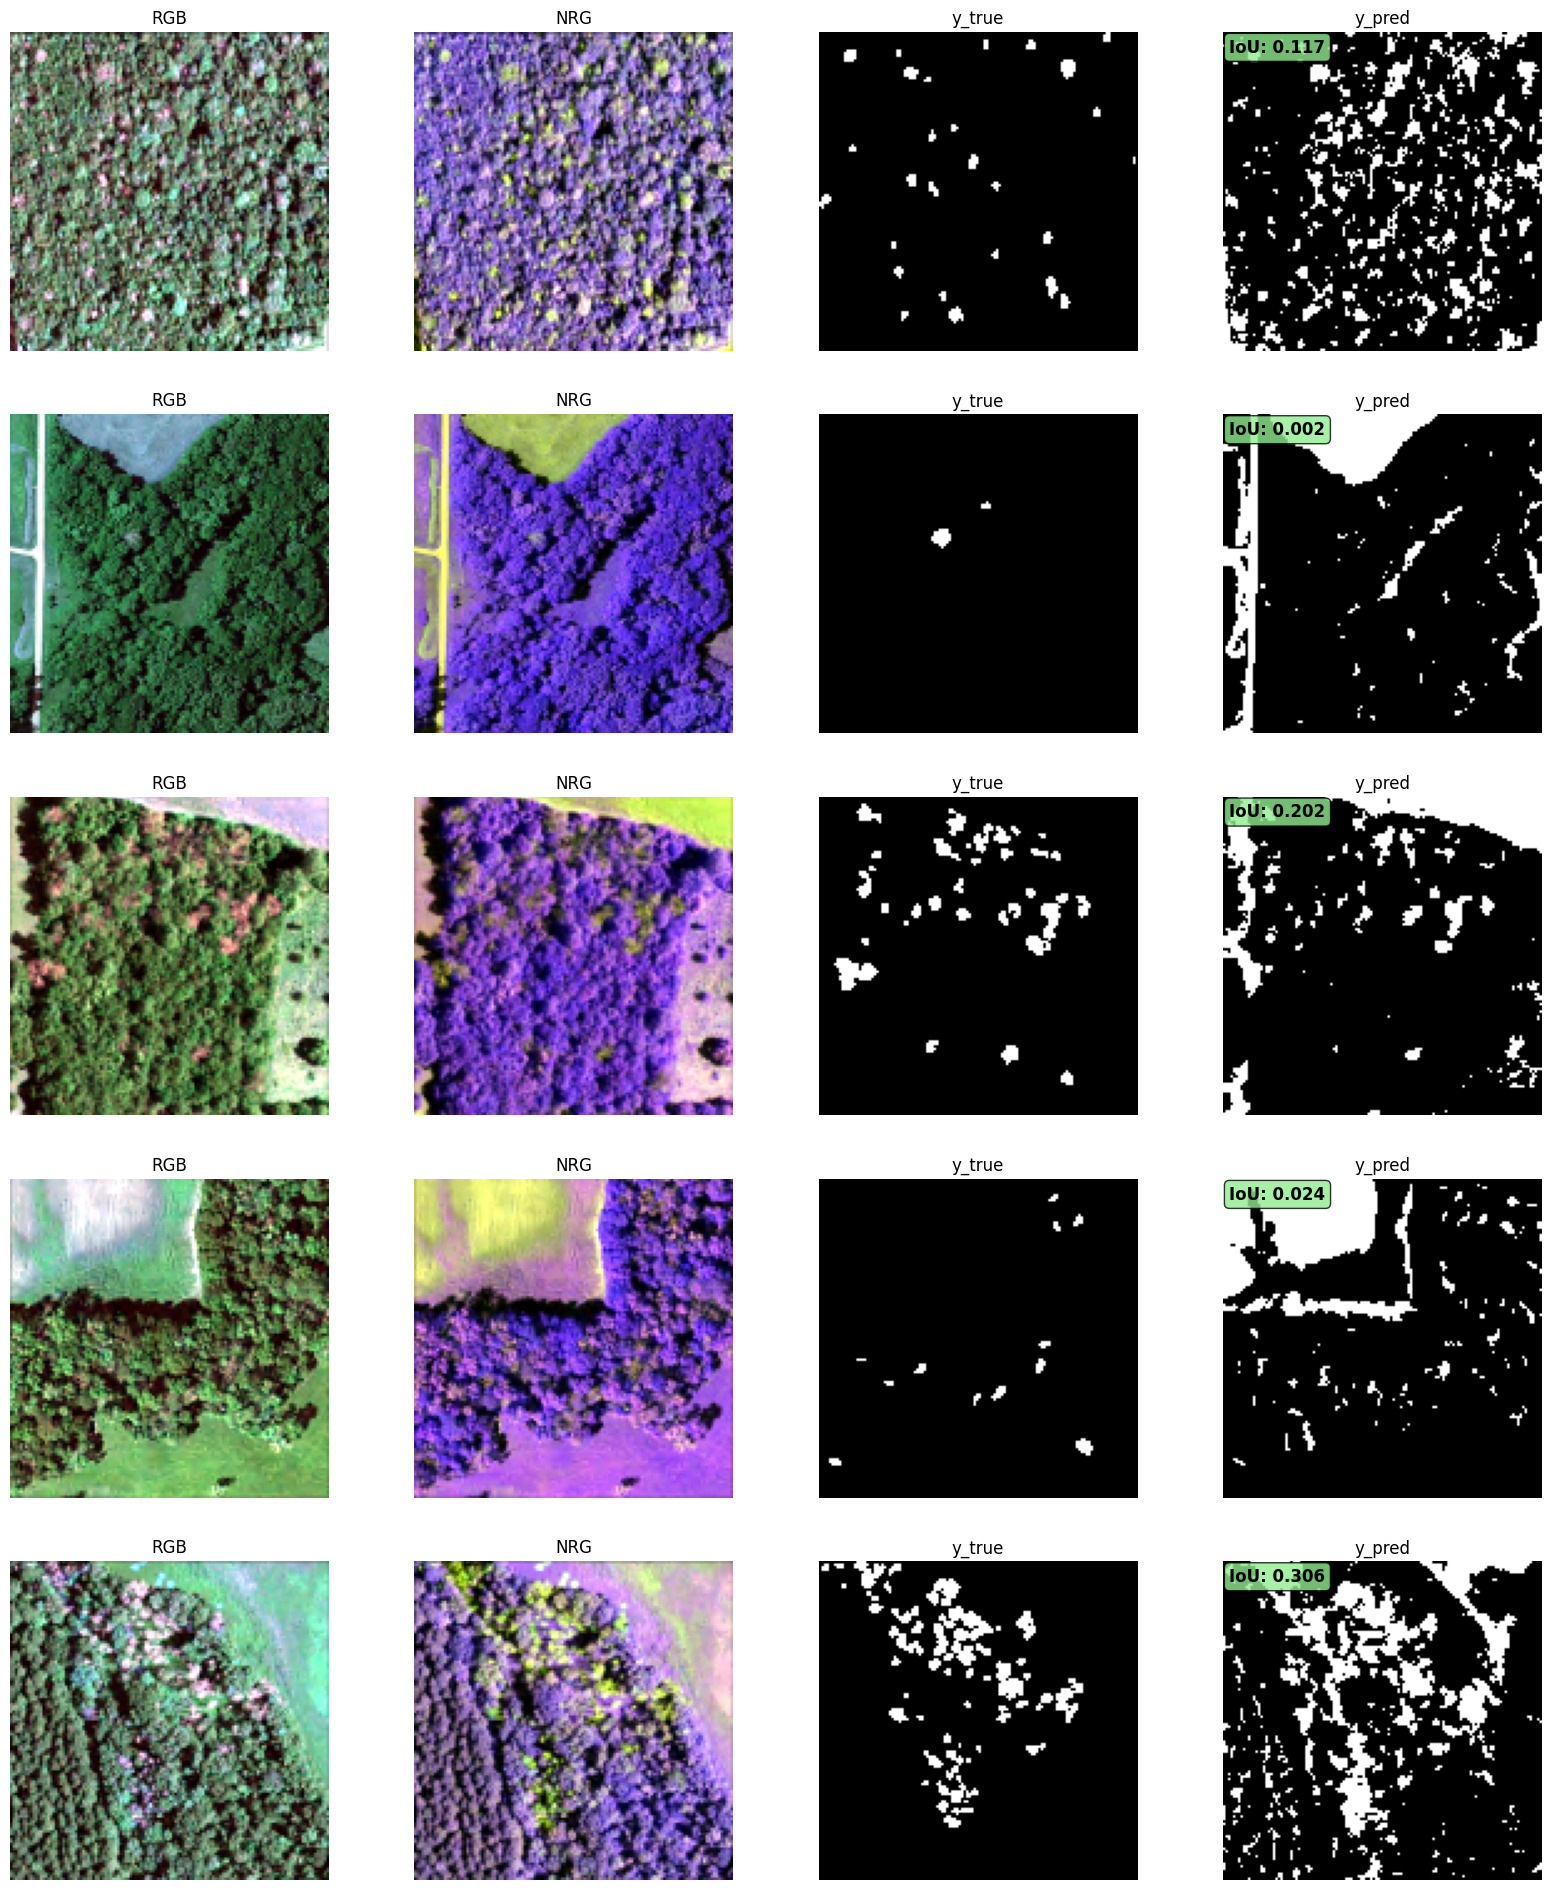
\includegraphics[width=.95\linewidth]{figs/SGDmask.jpg}\\
Upon looking at the prediction mask produced by the SGD classifier, it can immediately be seen that there is a striking contrast compared to the random forest classifier. There is a much higher recall rate with the SGD, however the false positive has also skyrocketed as the model is mis-classifying many of the background pixels as dead tree pixels (foreground).\\
There could be several explanations for this phenomenon; most notably, the dataset is quite imbalanced, the input images mostly consist of background pixels and the model could be overcompensating for the class imbalance by being bias towards making false positives.\\
Indeed, the model does actually perform somewhat better on images that have a higher concentration of dead tree pixels compared to images that have very few. Secondly, using only RGB/NRG pixel values is weak as it ignores spatial context and information, combining this with class imbalance makes it more difficult to differentiate between foreground and background pixels.\\
While the results are not very promising, there are considerable avenues in which the SGD model could be optimised, firstly a stricter threshold for predicting foreground pixels would likely reduce the false positive rate, extra features that capture local spatial information or texture (LBP/HoG) could help with more accurately differentiating foreground/background pixels.\\
The SGD model also trains considerably faster than the other models, able to reach convergence in seconds while the random forest model took significantly longer.
%\includegraphics[width=.95\linewidth]{figs/sgd-training.png}\\
\begin{lstlisting}[caption={SGD Training}, label={fig:sgd-train}]
-- Epoch 1
Norm: 1.49, NNZs: 6, Bias: -0.716938, T: 5455872, Avg. loss: 0.870819
Total training time: 0.62 seconds.
-- Epoch 2
Norm: 1.42, NNZs: 6, Bias: -0.554052, T: 10911744, Avg. loss: 0.572698
Total training time: 1.25 seconds.
-- Epoch 3
Norm: 1.53, NNZs: 6, Bias: -0.679788, T: 16367616, Avg. loss: 0.564680
Total training time: 1.89 seconds.
-- Epoch 4
Norm: 1.57, NNZs: 6, Bias: -0.654369, T: 21823488, Avg. loss: 0.561824
Total training time: 2.53 seconds.
-- Epoch 5
Norm: 1.50, NNZs: 6, Bias: -0.730205, T: 27279360, Avg. loss: 0.558549
Total training time: 3.17 seconds.
-- Epoch 6
Norm: 1.60, NNZs: 6, Bias: -0.806963, T: 32735232, Avg. loss: 0.557498
Total training time: 3.80 seconds.
-- Epoch 7
Norm: 1.61, NNZs: 6, Bias: -0.725729, T: 38191104, Avg. loss: 0.555748
Total training time: 4.44 seconds.
-- Epoch 8
Norm: 1.61, NNZs: 6, Bias: -0.692419, T: 43646976, Avg. loss: 0.556135
Total training time: 5.07 seconds.
-- Epoch 9
Norm: 1.60, NNZs: 6, Bias: -0.616872, T: 49102848, Avg. loss: 0.554584
Total training time: 5.71 seconds.
-- Epoch 10
Norm: 1.60, NNZs: 6, Bias: -0.598181, T: 54558720, Avg. loss: 0.554805
Total training time: 6.35 seconds.
-- Epoch 11
Norm: 1.62, NNZs: 6, Bias: -0.689664, T: 60014592, Avg. loss: 0.554993
Total training time: 6.98 seconds.
-- Epoch 12
Norm: 1.62, NNZs: 6, Bias: -0.618751, T: 65470464, Avg. loss: 0.553864
Total training time: 7.61 seconds.
-- Epoch 13
Norm: 1.59, NNZs: 6, Bias: -0.656321, T: 70926336, Avg. loss: 0.554055
Total training time: 8.25 seconds.
-- Epoch 14
Norm: 1.65, NNZs: 6, Bias: -0.698402, T: 76382208, Avg. loss: 0.555047
Total training time: 8.88 seconds.
Convergence after 14 epochs took 8.88 seconds
\end{lstlisting}

\subsection{SVM}
Unfortunately, we were unable to train a SVM classifier given that the small feature space relative to the size of the dataset. Recall that each training sample is a 6-dimensional vector that corresponded to a dead tree pixel or a background pixel. Given the size of the training data and the fact the classes were quite imbalanced, it was not possible to find a hyperplane that reasonably separated pixels into the 2 categories.\\


\subsection{CNN}
To address class imbalance and enhance segmentation quality, a loss function combines binary Cross-Entropy and Dice Loss. The adam optimizer effectively minimized the hybrid loss through adaptive learning rate adjustment. Compared to the results, the simple CNN model achieved higher precision than the encoder-decoder model, which IoU are 0.28 and 0.16 separately. However, the encoder-decoder model has significantly faster training speeds and testing times. Notably, RGB inputs consistently outperformed NIR-only data across both models, though the RGB+NIR combination provided marginal improvements over RGB alone in the simple CNN. These findings suggest a fundamental trade-off between segmentation accuracy and computational efficiency in this method. 
\begin{lstlisting}[language=Python]
def dice_loss(y_true, y_pred, smooth=1e-6):
    y_true_f = tf.reshape(y_true, [-1])
    y_pred_f = tf.reshape(y_pred, [-1])
    intersection = tf.reduce_sum(y_true_f * y_pred_f)
    return 1 - (2. * intersection + smooth) / (tf.reduce_sum(y_true_f) + tf.reduce_sum(y_pred_f) + smooth)

def combo_loss(y_true, y_pred):
    bce = tf.keras.losses.binary_crossentropy(y_true, y_pred)
    return bce + dice_loss(y_true, y_pred)
\end{lstlisting}
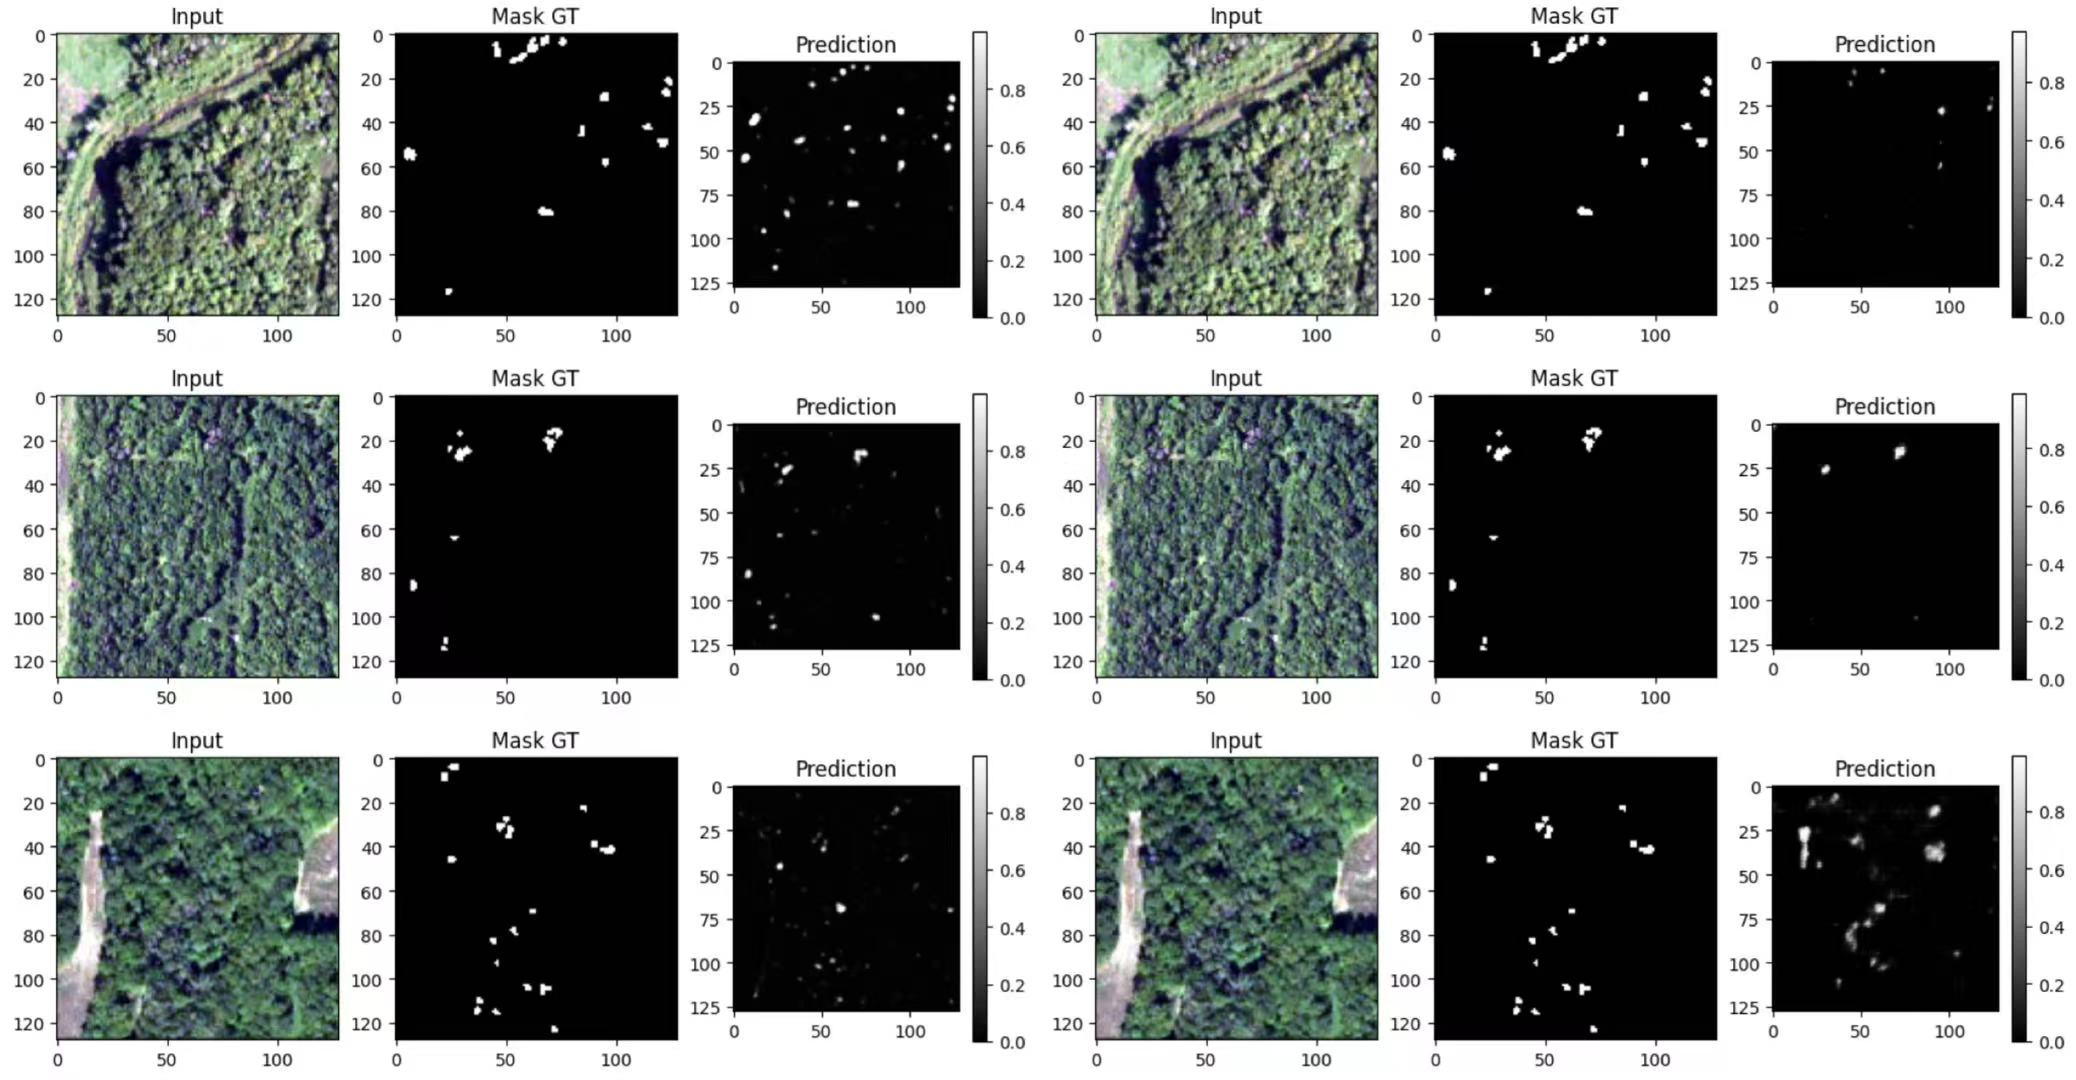
\includegraphics[width = 9cm]{figs/CNN_mask.jpg}\\
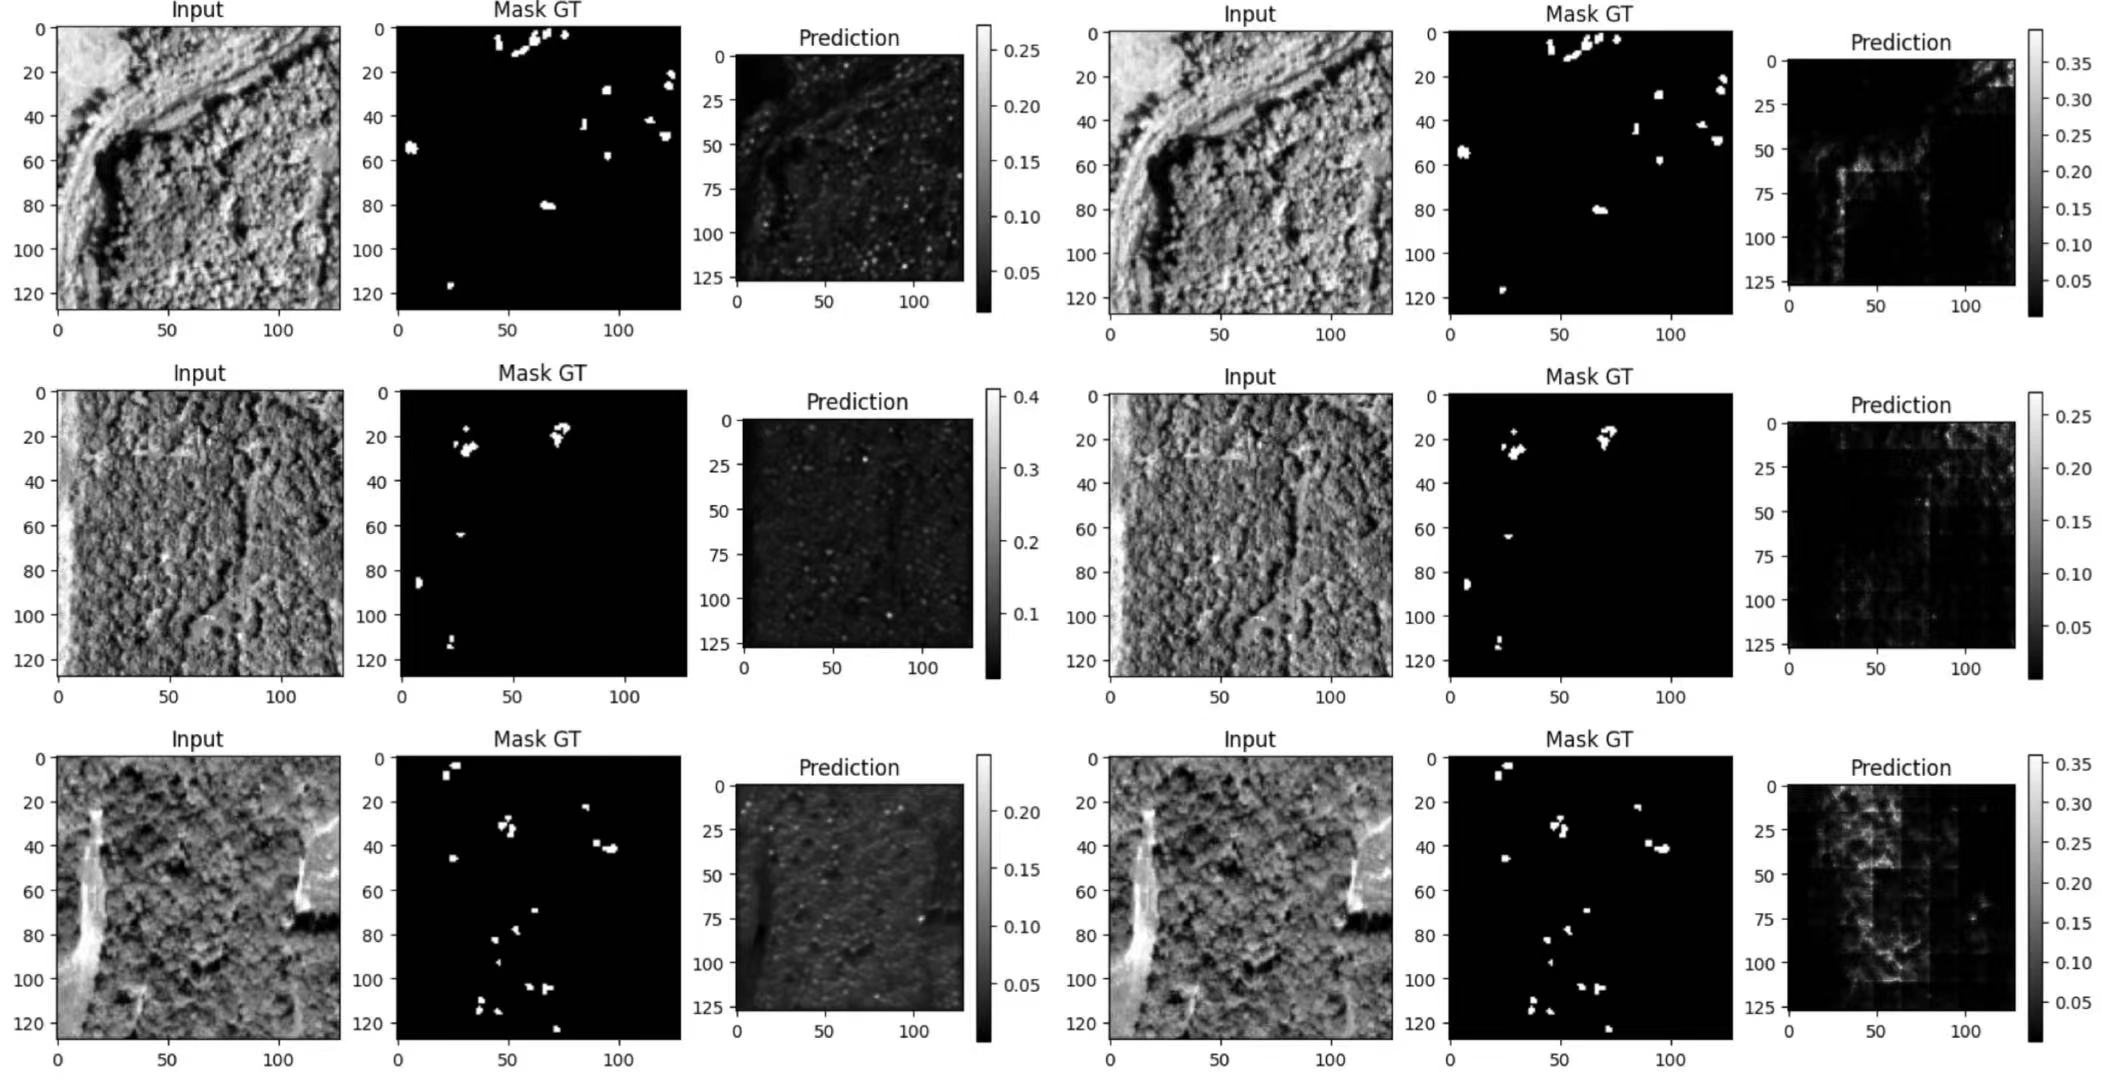
\includegraphics[width = 9cm]{figs/CNN_mask2.jpg}\\
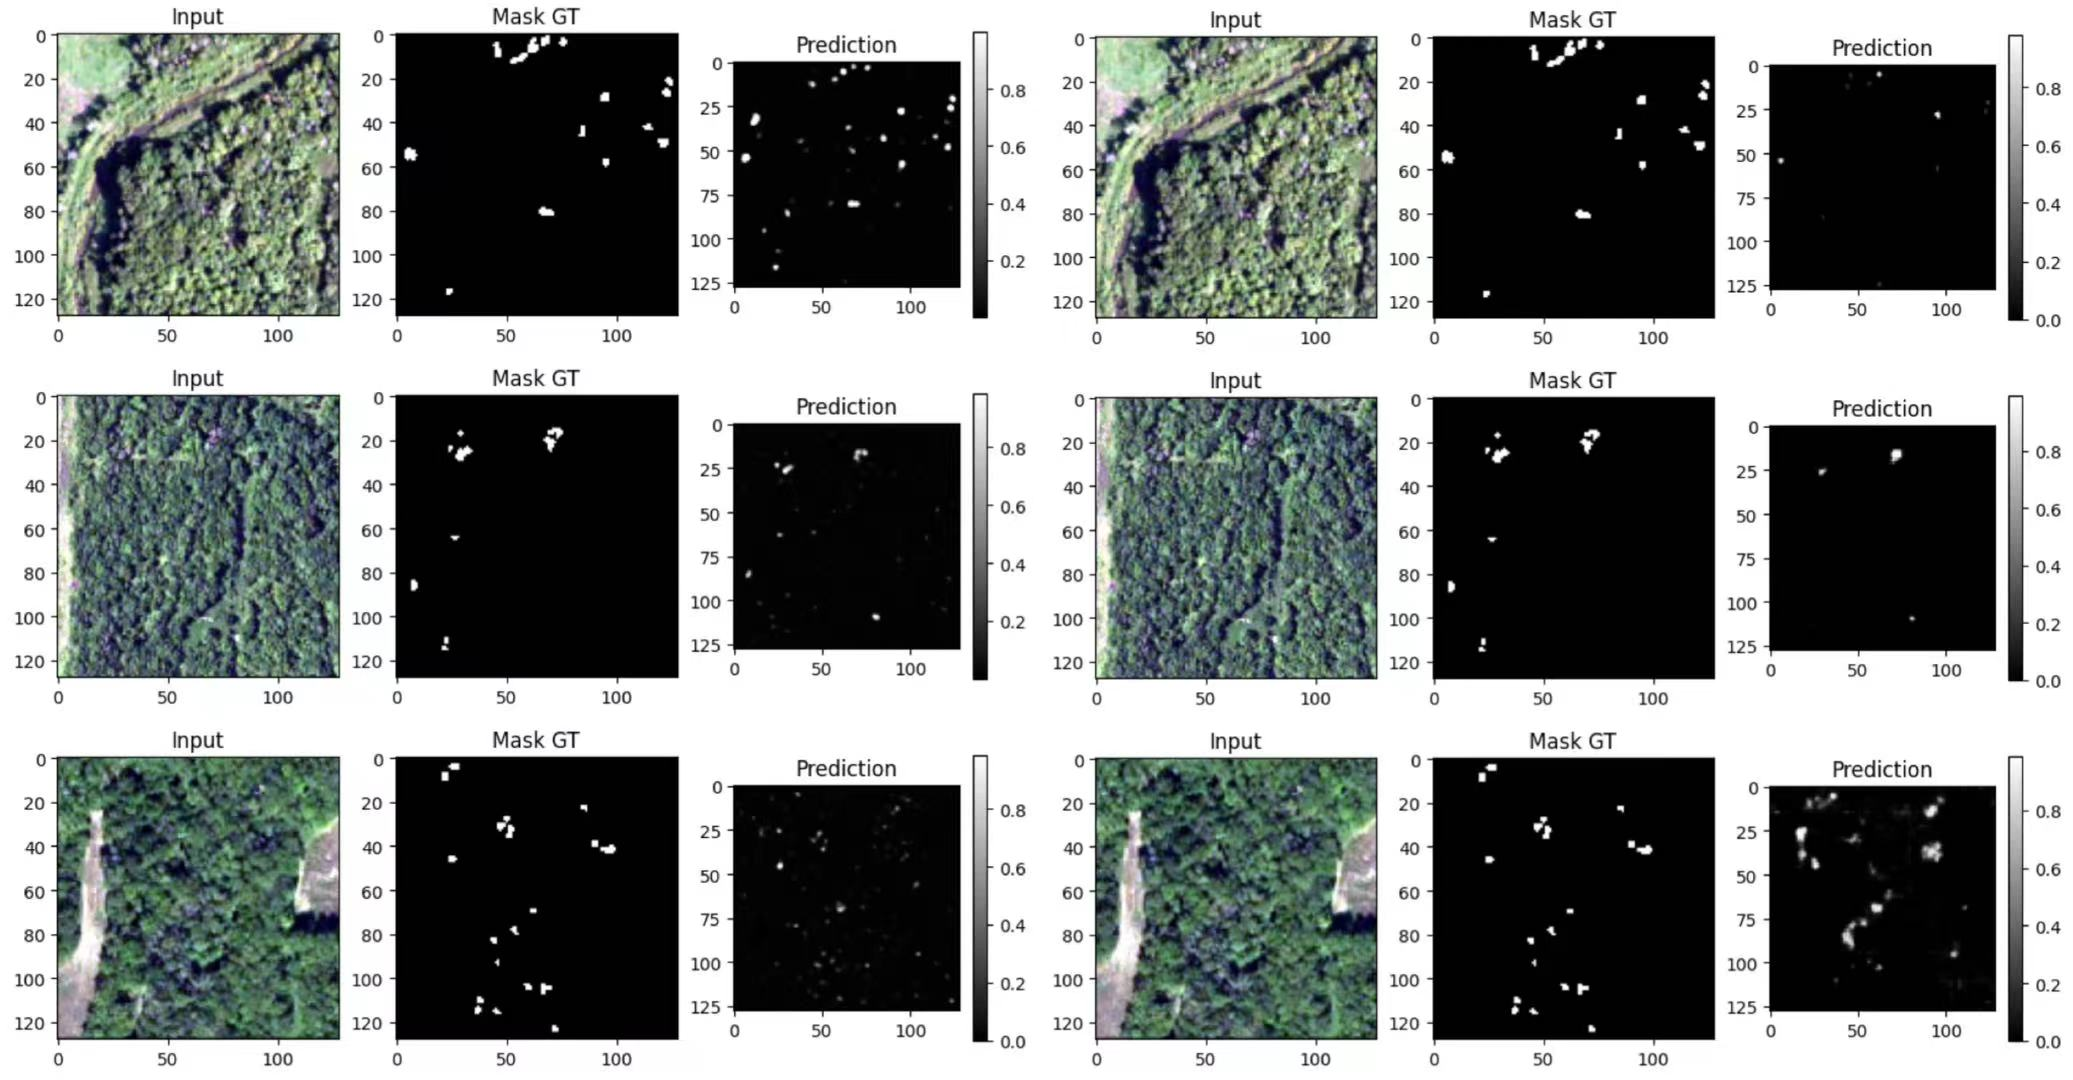
\includegraphics[width = 9cm]{figs/CNN_mask3.jpg}\\
% that's better jing jing, do you mind adding captions so it doesn't look like 1 huge image?
\subsection{CBAM}
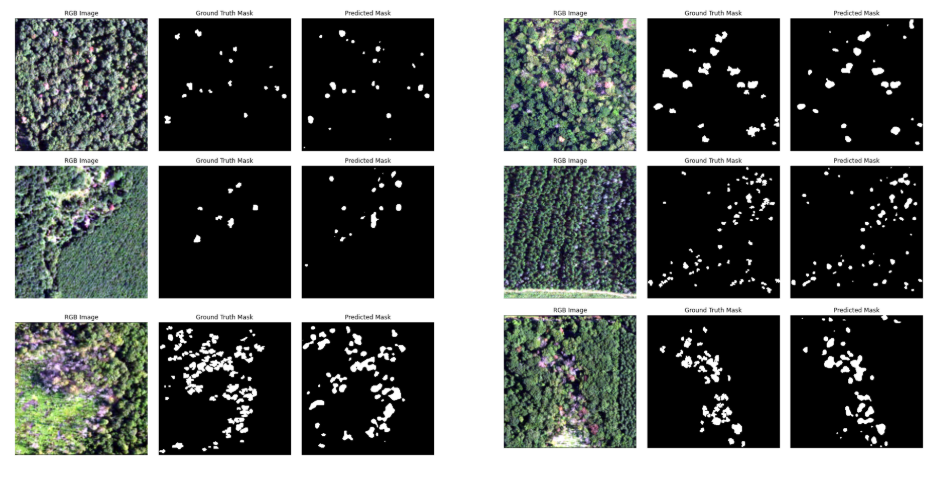
\includegraphics[width=1\linewidth]{figs/DeepLabExample.png}
\paragraph{Backbone depth.}
Replacing ResNet‐18 with deeper variants (ResNet‐50 and ResNet‐101) does \emph{not}
translate into higher accuracy: mIoU changes by \(+0.2\) pp and \(-0.1\) pp,
respectively, which is within statistical noise.
The likely reason is that the training set (444 images) is too small for parameters to be learnt properly; they converge to a poor local minimum in which both training and validation predictions are nearly constant.

\paragraph{Augmentation intensity.}
A controlled sweep over augmentation strength shows a bell-shaped trend:
\emph{mild} transforms (flip, \(\pm30^\circ\) rotation) add \(+\!1.3\) mIoU, but \emph{aggressive} settings (\(\pm45^\circ\) rotation, Cutout 40 \%, Gaussian blur \(\sigma{=}3\)) drop performance by \(3.7\) pp.
Excessive geometric distortion breaks the thin‐structure prior that the
network needs to recognise dead branches, while heavy photometric jitter
destroys the cross-spectral cues learned from the NIR and visible bands.

\subsection{UNet}
\label{sec:aj_unet_discussion}

Our UNet implementation achieved a final IoU of 0.7078 through careful architectural choices and domain-specific engineering. We spend this section on analysing the key design decisions and their impact on segmentation performance.

\paragraph{Double Convolution Benefits.}
The DoubleConvolution module forms the backbone of our encoder-decoder architecture, applying two consecutive 3×3 convolutions with ReLU activations:

\begin{lstlisting}[language=Python]
class DoubleConvolution(nn.Module):
    def __init__(self, in_channels: int, out_channels: int):
        super().__init__()
        self.first = nn.Conv2d(in_channels, out_channels, kernel_size=3, padding=1)
        self.act1 = nn.ReLU()
        self.second = nn.Conv2d(out_channels, out_channels, kernel_size=3, padding=1)
        self.act2 = nn.ReLU()
\end{lstlisting}

The implementation was naïvely thieved from a reference in the Course Slides \cite{b19}, however the code later proved to be good. The double convolution provided advantages over single convolutions. First, the increased receptive field (5×5 effective) captured larger spatial patterns whilst maintaining parameter efficiency compared to direct 5×5 kernels. Second, the intermediate activation introduces non-linearity (as mentioned in the presentation) that enhances the network's capacity to learn complex feature representations. Most critically for dead tree segmentation, the double convolution enabled detection of thin branching structures that require multiple scales of spatial reasoning. Single 3×3 kernels are less capable of capturing the elongated, irregular shapes characteristic of dead tree canopies \cite{b20}.

\paragraph{Connected Components Post-Processing Limitations.}
Initial experiments included connected components analysis to remove the salt and pepper (loosely speaking) false positives, and enforce spatial coherence. However, this approach proved counterproductive for our domain:

\begin{lstlisting}[language=Python]
# abandoned connected components approach
def apply_connected_components(predictions, min_component_size=50):
    # removes components smaller than threshold
    # problem: Dead trees often appear as multiple small components
    # due to sparse branching patterns
    pass
\end{lstlisting}

Dead trees exhibit highly fragmented spatial distributions—individual trees often appear as collections of thin branches separated by gaps, rather than contiguous blobs. Connected components filtering eliminated these legitimate small structures, reducing recall significantly. The morphological operations (opening and closing) proved superior as they preserve connectivity while removing noise, respecting the natural fragmentation of dead tree structures. Experimenting with a mixed loss also helped.

\paragraph{Binary Cross-Entropy Training Instability.}
Early training attempts using only Binary Cross-Entropy loss resulted in highly unstable convergence, as shown in Figure \ref{fig:bad_training}:

\begin{figure}[h]
  \centering
  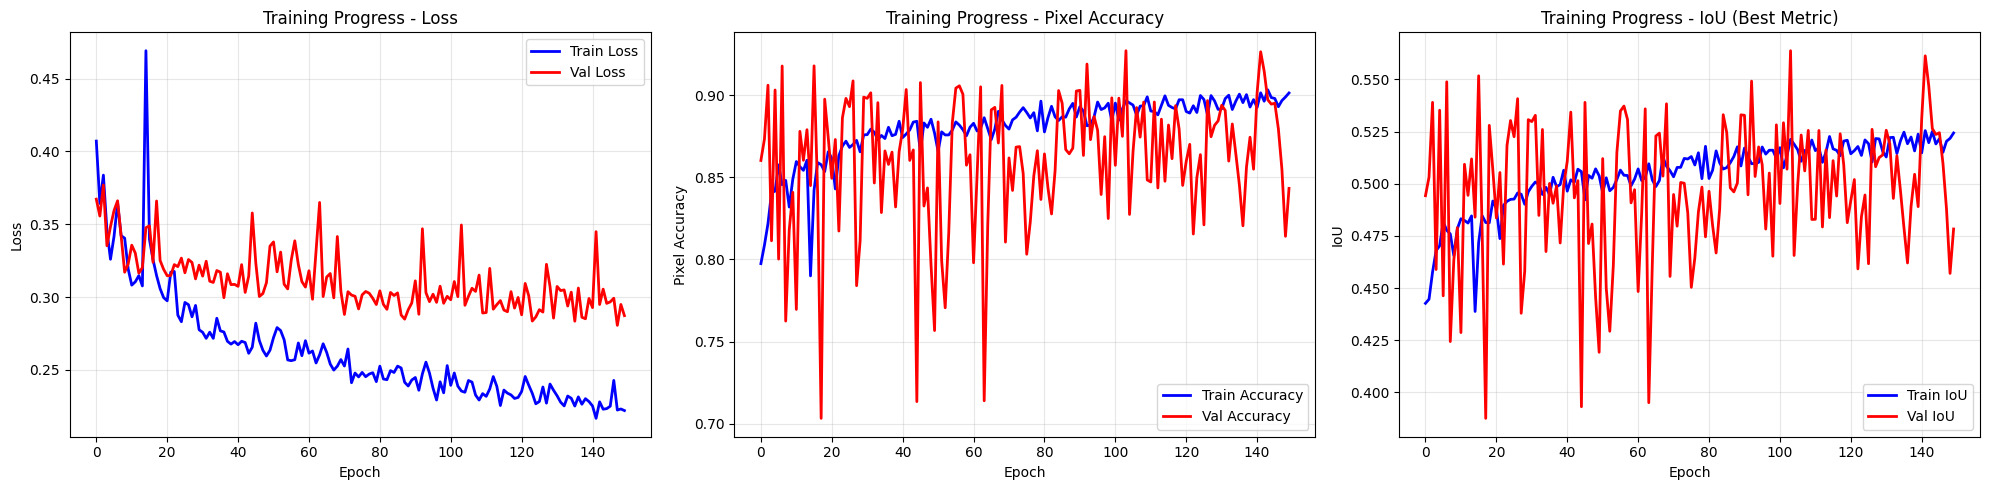
\includegraphics[width=0.9\linewidth]{figs/unet-bad-train.jpg}
  \caption{Training instability with BCE-only loss showing erratic convergence and suboptimal final performance}
  \label{fig:bad_training}
\end{figure}

The extreme class imbalance (97\% background pixels) caused the network to exploit the trivial solution of predicting background everywhere, achieving high pixel accuracy (0.97) but zero IoU. The loss function oscillated wildly as the network alternated between this degenerate solution and attempting to learn meaningful features. The combined Dice-Focal loss resolved this by directly optimising IoU-related metrics while down-weighting easy negative examples, leading to stable convergence and meaningful dead tree detection.

\paragraph{Performance Comparison: BCE vs. Combined Loss.}
Figure \ref{fig:loss_comparison} demonstrates the dramatic improvement achieved through our composite loss function:

\begin{figure}[htbp]
  \centering
  \begin{minipage}{0.47\linewidth}
    \centering
    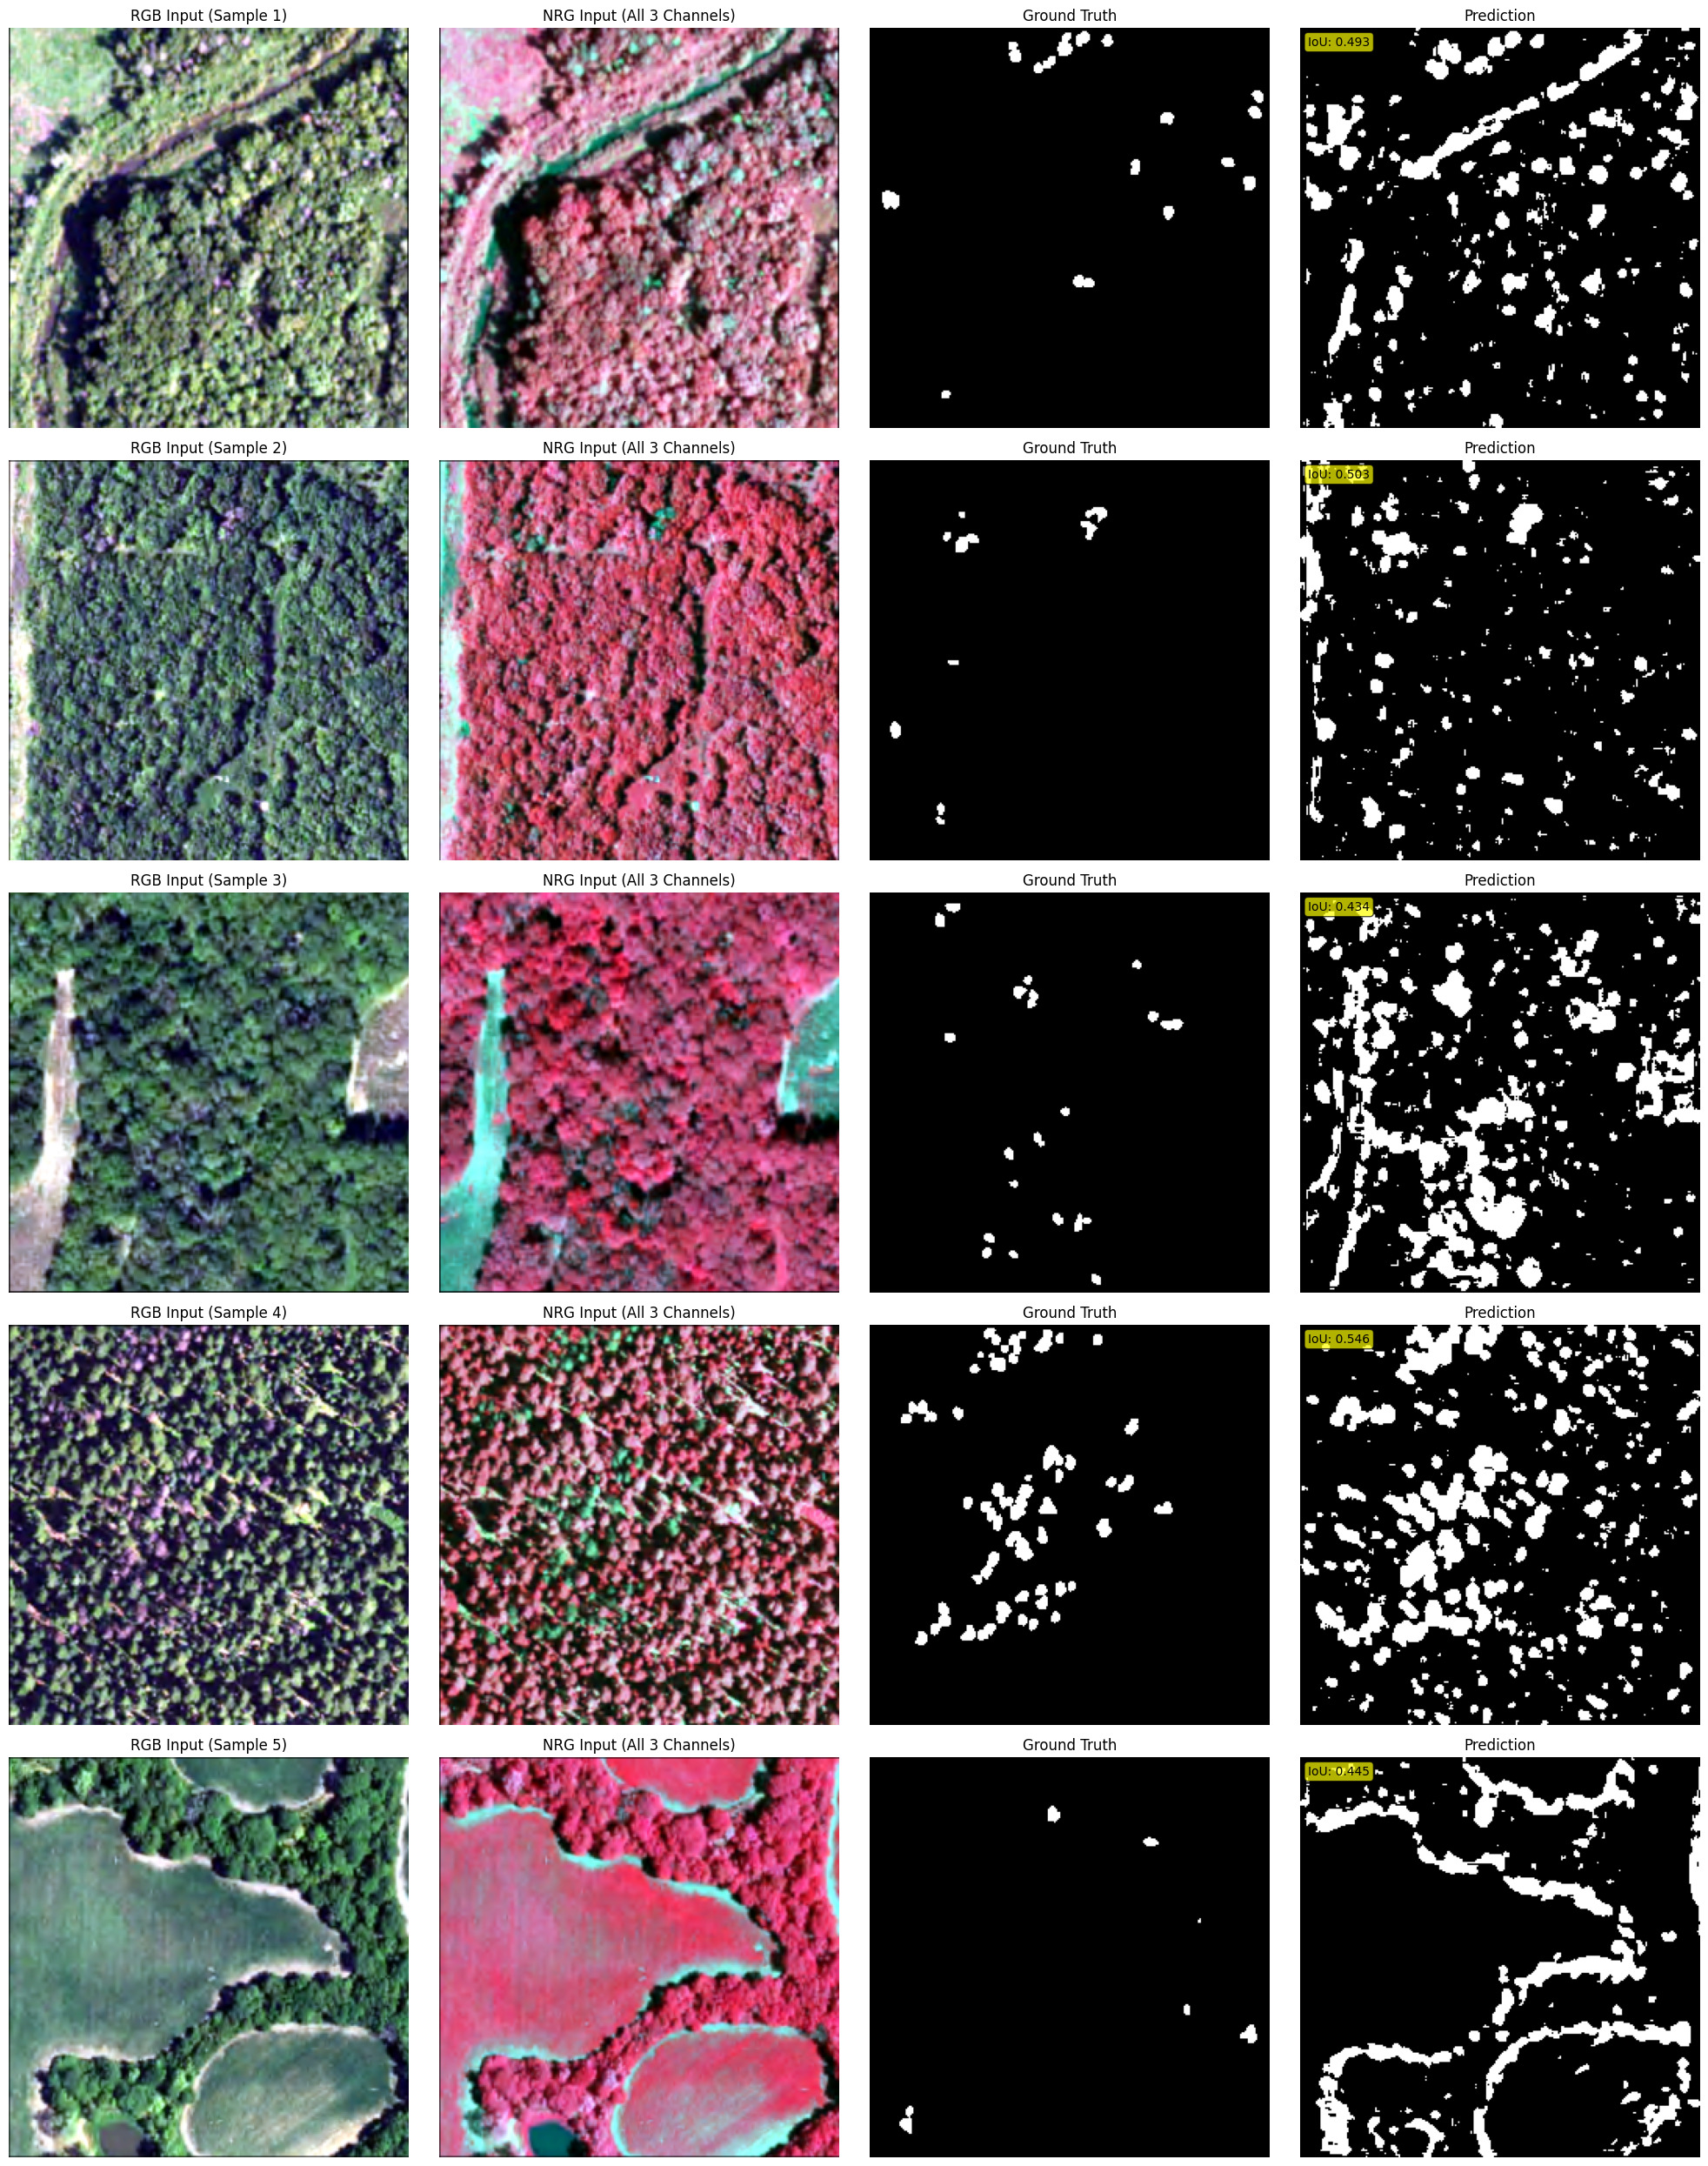
\includegraphics[width=0.9\linewidth]{figs/unet-bad-result-grid.jpg}
    \subcaption{BCE loss (IoU 0.12)}\label{fig:bad}
  \end{minipage}\hfill
  \begin{minipage}{0.47\linewidth}
    \centering
    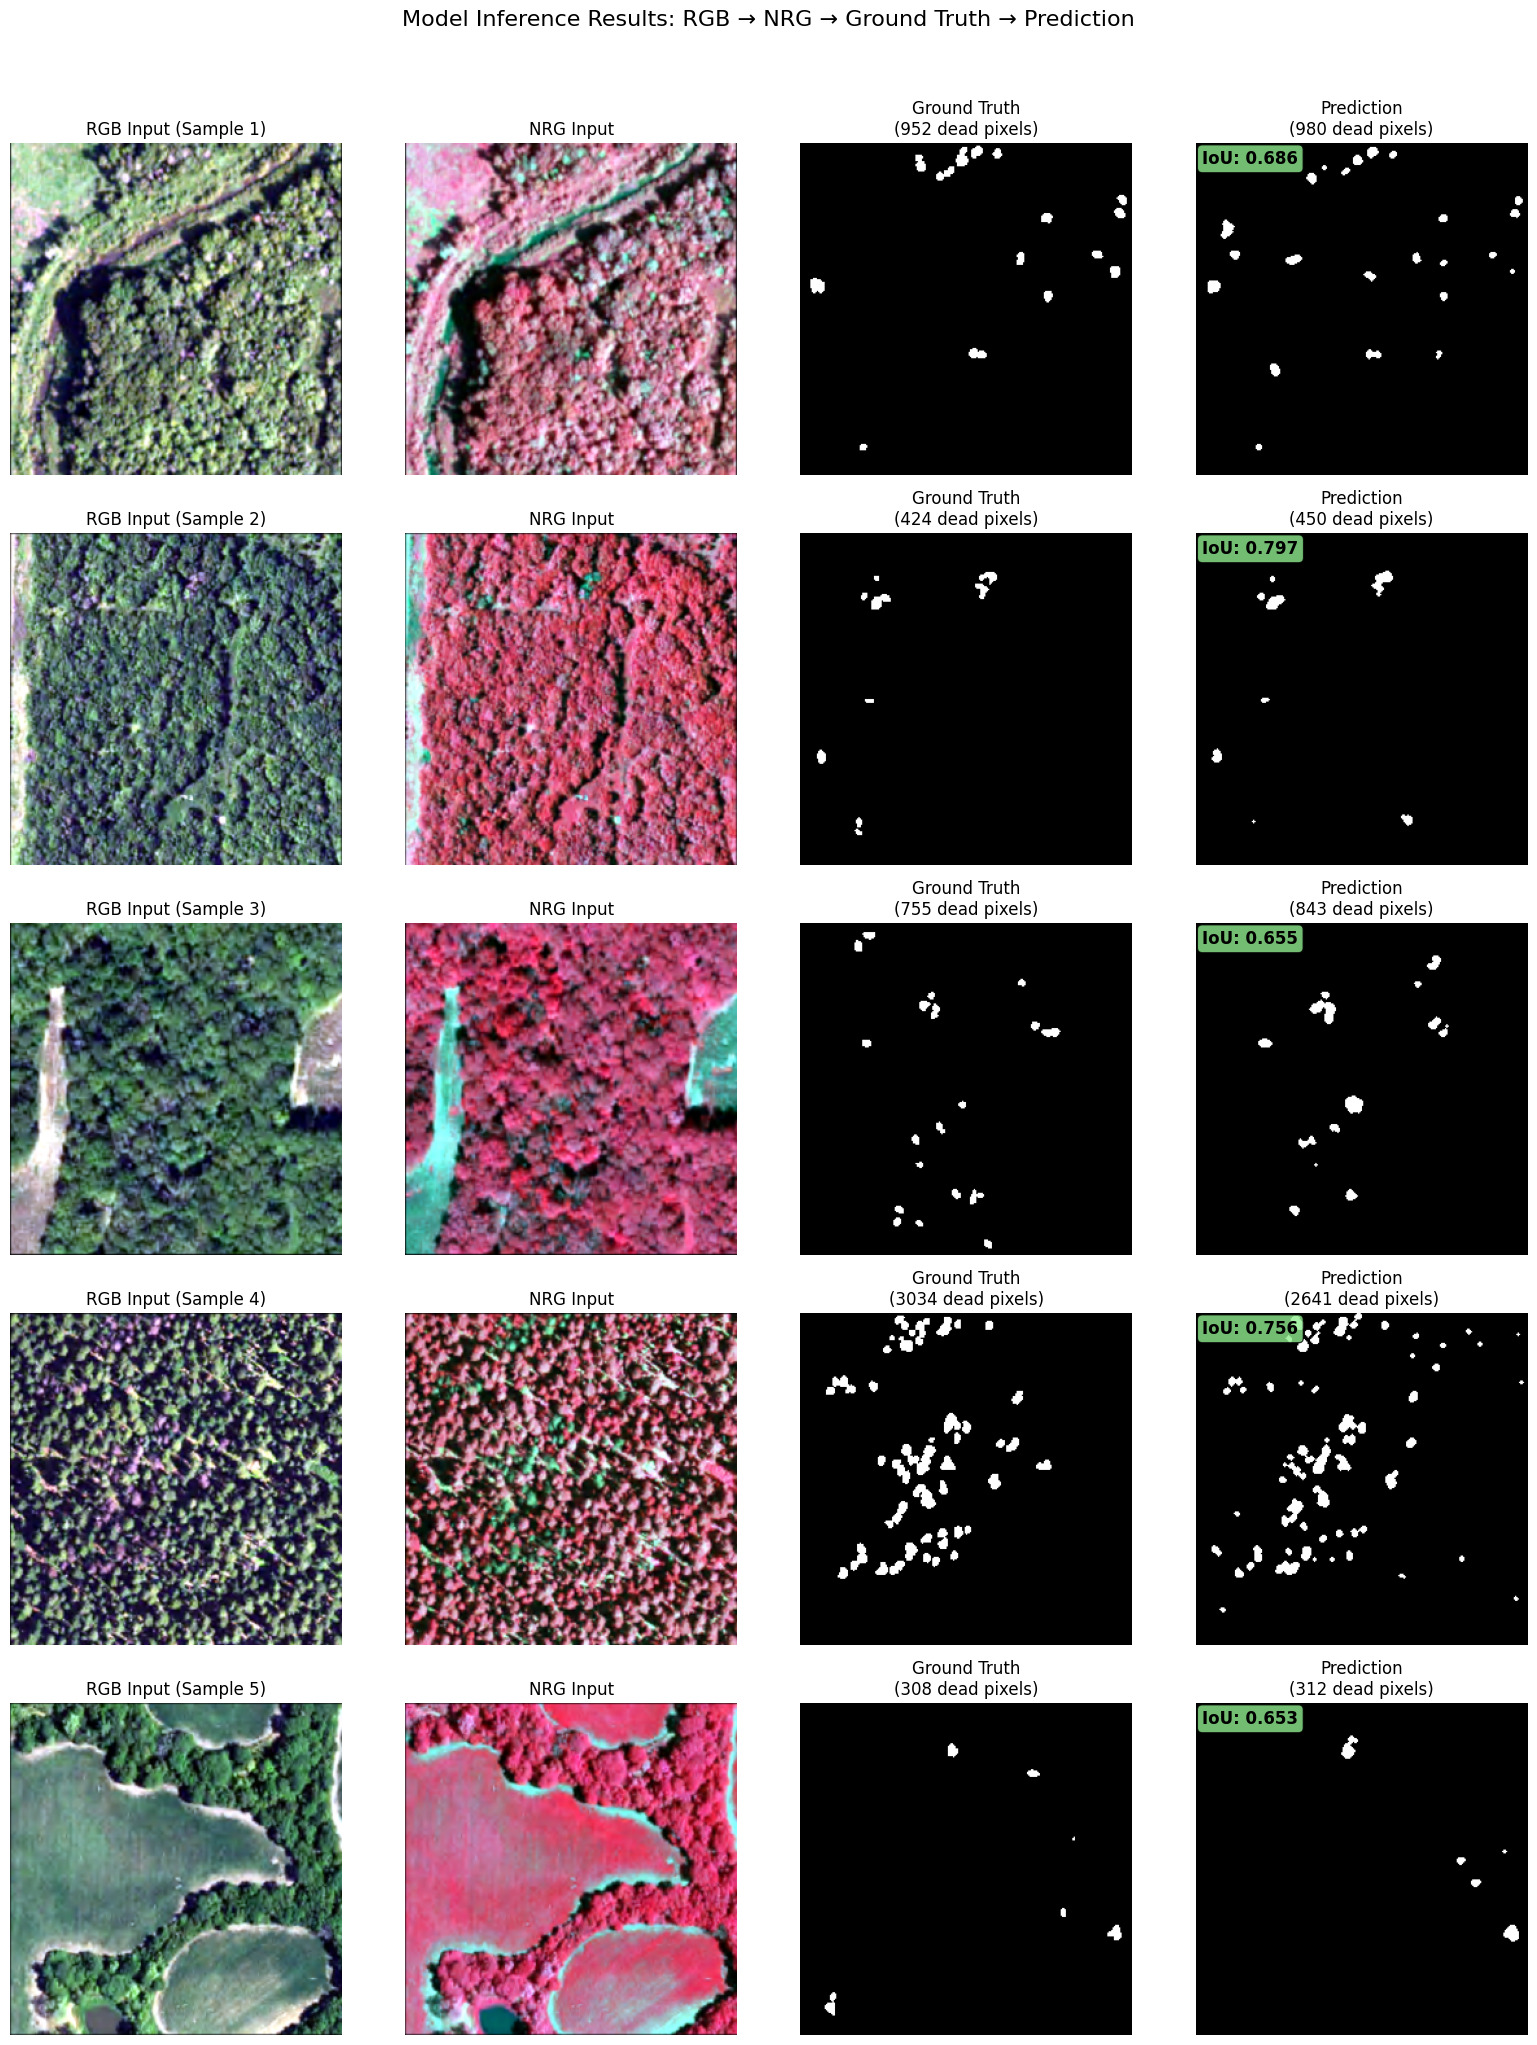
\includegraphics[width=0.9\linewidth]{figs/unet-good-result-grid.jpg}
    \subcaption{Dice + Focal (IoU 0.71)}\label{fig:good}
  \end{minipage}
  \caption{Segmentation quality comparison: BCE-only training produces sparse predictions (a) whereas the combined Dice–Focal loss yields coherent dead-tree masks (b).}
  \label{fig:loss_comparison}
\end{figure}

The BCE-only model produces sparse, disconnected predictions that fail to capture tree structures, while our combined loss generates coherent segmentations that accurately delineate dead tree boundaries.

\paragraph{Parameter Counts.}
The UNet implementation contains 31,042,434 parameters, distributed across the encoder-decoder hierarchy:

\begin{lstlisting}[language=Python]
print(f"UNET PARAMETERS: {sum(p.numel() for p in model.parameters()):,}")
> DEVICE: cuda
> UNET PARAMETERS: 31,034,690
\end{lstlisting}

This substantial parameter count demonstrates the robustness of this architecture compared to our other approaches. The simple CNN model, with only 4 convolutional layers and [32, 64, 128, 256] filters, contains approximately 2-3M parameters yet achieves only IoU = 0.286. Similarly, the DeepLabV3+ with CBAM model, built on a ResNet-18 backbone (~11M base parameters) with attention mechanisms and ASPP modules, totals roughly 15-18M parameters but reaches only IoU = 0.400.

The 31M-parameter UNet model however, achieves an IoU of 0.705—a 76\% improvement over CBAM and 146\% over the simple CNN! This performance gap justifies the increased parameter count: the encoder-decoder symmetry with skip connections requires substantial parameter investment, but enables precise boundary localisation that smaller networks cannot achieve. 

Furthermore, our model avoids the overfitting that plagued deeper CBAM variants (ResNet-50/101 showed no improvement), suggesting our parameter allocation is well-suited to the 355-image training set. 

\paragraph{Colour Jittering Abandonment.}
Initial data augmentation included colour jittering to improve generalisation:

\begin{lstlisting}[language=Python]
# orphaned augmentation approach
transforms.ColorJitter(brightness=0.2, contrast=0.2, saturation=0.2, hue=0.1)
\end{lstlisting}

We abandoned this pretty quick because it was a transformation that would only apply to the RGB channels and we wished to train on NIR too.
Colour jittering disrupts the spectral relationships so instead, we employed geometric augmentations (flips, rotations) that preserve spectral integrity while providing spatial generalisation.

\begin{lstlisting}[language=Python]
if augment:
    base_transforms.extend([
        T.RandomHorizontalFlip(p=0.5),
        T.RandomVerticalFlip(p=0.5),
        T.RandomRotation(10),
    ])
\end{lstlisting}


\paragraph{Final Architecture Performance.}
The optimised UNet architecture achieved robust performance across diverse test conditions, with post-processing providing consistent improvements. The 8-channel input pipeline, combined with the composite loss function and carefully selected augmentations, enabled effective dead tree segmentation despite significant class imbalance and complex spatial structures. The final IoU of 0.7078 represents a substantial improvement over baseline approaches and demonstrates the value of domain-specific architectural choices in challenging segmentation tasks.
